\documentclass[letterpaper]{report}

\usepackage[utf8]{inputenc}  % Ng Edit for accents in Spanish
\usepackage[spanish]{babel}  % Ng Edit for accents in Spanish
\usepackage{hyperref}        % Ng Edit for adding urls
\usepackage{graphicx}        % Ng Edit for adding graphics
\usepackage{setspace}
\usepackage{amsmath}
\usepackage{algpseudocode}
\usepackage{algorithm}

%Path relative to the .tex file containing the \includegraphics command
\graphicspath{ {img/} }
\algnewcommand\algorithmicforeach{\textbf{for each}}
\algdef{S}[FOR]{ForEach}[1]{\algorithmicforeach\ #1\ \algorithmicdo}

\def\equationautorefname~#1\null{(#1)\null} %to use parenthesis in eqs.
\onehalfspacing
\title{\bf
  Mejora en la optimización de la ubicación de trampas para mosquito con
  Particle Swarm Optimization.
}

\author{Topiltzin Hernández Mares}

\begin{document}

\maketitle
\thispagestyle{empty}
\pagestyle{empty}
\tableofcontents
\listoffigures
\listoftables

% \begin{abstract}
% \end{abstract}

% \chapter{Introducción}

\chapter{Estado del arte}
  Antes de hablar del problema y su solución, es necesario entrar en contexto.
  Por esto, en la primera sección de este capítulo se definirán conceptos
  básicos, tales como trampas para mosquitos, las cuales tienen un papel central
  en el problema. Enseguida, se hablará sobre términos de inteligencia
  artificial y métodos de optimización, los cuales ayudarán a entender mejor las
  problemática y su solución.
  
  En la segunda parte de este capítulo se hablará de algunos trabajos recientes
  para poder entender el estado del arte en problemas de optimización. Sin
  embargo, por la poca investigación relacionada a la optimización de vigilancia
  de mosquitos, se analizarán trabajos similares enfocados en redes y
  monitoreo.

\section{Conceptos básicos}
  En este trabajo se tocan temas de optimización, que es una de las ramas de la
  inteligencia artificial, por lo que es conveniente definir algunos conceptos
  importantes antes de continuar. 

  \subsection{Inteligencia artificial}
    En el libro Artificial Intelligence: A Modern Approach
    \cite{AIModernAproach}, se define la inteligencia artificial (IA) como
    máquinas con pensamiento parecido al humano y con acciones racionales.
    
    Una definición más elaborada es la de \cite{AIDef}: IA es un término
    utilizado para etiquetar a computadoras que imitan funciones humanas
    cognitivas, tales como aprendizaje y resolución de problemas. De igual
    manera, se llama inteligencia artificial a algoritmos que trabajan con la
    misma complejidad que expertos humanos.
  
  \subsection{Optimización}
    Puede ser definida como el proceso de encontrar la mejor solución posible
    entre todas las disponibles. Por lo tanto, la tarea de optimización es
    modelar algún problema en términos de alguna función de evaluación y emplear
    algún algoritmo de búsqueda para minimizar (o maximizar) esa función
    objetivo. Sin embargo, no es posible asegurar que el resultado óptimo será
    encontrado, ya que hay problemas demasiado grandes que es imposible
    encontrar la solución óptima \cite{SearchMethodologies}.
  
  \subsection{Heurísticas}
    En el área computacional de optimización, se llaman heurísticas a los
    métodos usados para buscar soluciones de alta calidad, sin asegurar la
    óptima.

    Una definición más elaborada la da \cite{HeuristicDef}, pues dice
    que una técnica heurística es un método que busca soluciones buenas (y casi
    óptimas) con un costo computacional bajo. Sin embargo, estos métodos no son
    capaces de indicar qué tan cerca de la optimización perfecta se encuentra 
    la respuesta actual dada por una heurística.
  
  \subsection{Metaheurísticas}
    Se refiere a técnicas que coordinan, manipulan y guían el comportamiento y
    soluciones de métodos heurísticos de optimización. Tales métodos pueden ser
    desde procedimientos de alto nivel o pueden describir las alteraciones
    posibles para una heurística \cite{MetaheuristicsDef}.

    Existe una gran cantidad de metaheurísticas
    \cite{HeuristicDef, SearchMethodologies}, más adelante se hablará de algunos
    métodos, tal como algoritmos genéticos y optimización de enjambre de
    partículas.
  
  \subsection{Inteligencia de enjambre}
    La inteligencia de enjambre es un campo computacional que diseña y estudia
    algoritmos para buscar soluciones a problemas. Estos algoritmos están 
    inspirados en el comportamiento complejo y, algunas veces, coordinado de
    enjambres de cualquier organismo natural \cite{SearchMethodologies}. 
    
    \begin{figure}[ht!]
      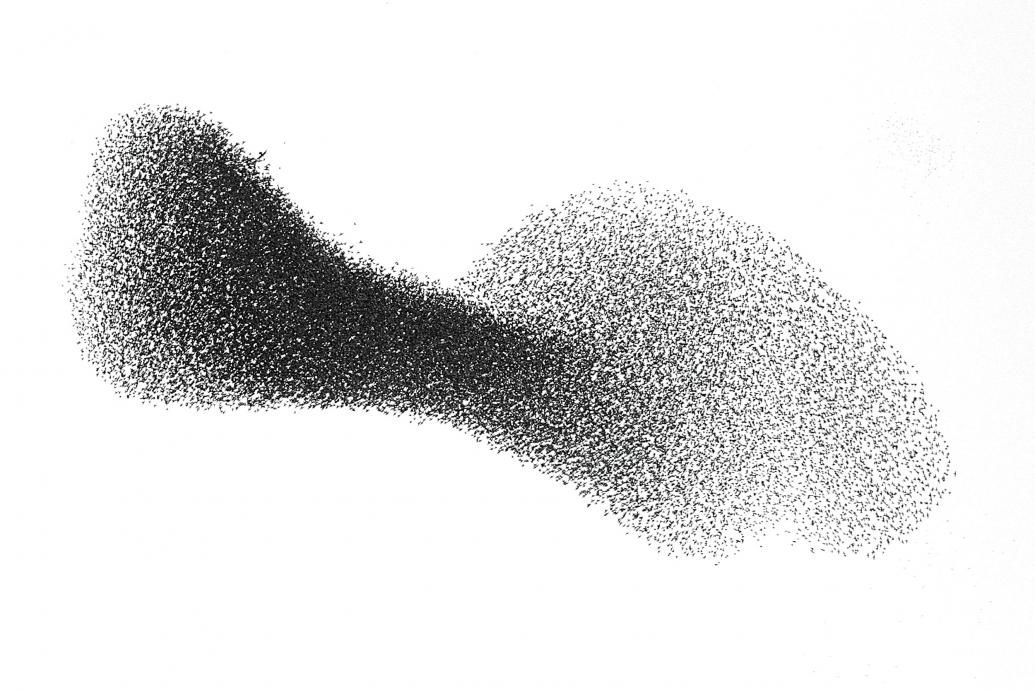
\includegraphics[scale=0.18]{si-repr}
      \centering
      \caption{Inspiración de algoritmos de inteligencia de enjambre.}
      \centering
    \end{figure}

  \subsection{Algoritmos evolutivos}
    Son un tipo de algoritmos que buscan soluciones a problemas, tomando
    inspiración de la selección natural y genética \cite{EADef,GADef}. Estos 
    algoritmos pueden representar cromosomas como cadenas de texto, los cuales 
    son las soluciones a los problemas; los alfabetos representan genes; y más
    conceptos tomados de la biología.

  \subsection{Particle Swarm Optimization}\label{subsec:pso}
    Particle Swarm Optimization (PSO) fue inventada por Eberhart y Kennedy en
    1995 \cite{PSODef}, es un algoritmo
    estocástico inspirado en el comportamiento de una parvada de aves en busca
    de alimento. Cada partícula en el algoritmo, que representa una solución al
    problema, vuela en el espacio de búsqueda, actualizando su velocidad y su
    posición. La ecuación clásica para actualizar la velocidad de una partícula
    es \ref{eq:1} y para actualizar su posición es \ref{eq:2}.

    \begin{equation}
      \label{eq:1}
      v_{ij} = v_{ij} + c_1 rand()(p_{ij} - x_{ij}) + c_2 rand()(p_{nj} - x_{ij})
    \end{equation}

    \begin{equation}
      \label{eq:2}
      x_{ij} = x_{ij} + v_{ij}
    \end{equation}

    Actualmente, el algoritmo PSO canónico (CPSO) o PSO con peso inercial
    (PSO-iw) es considerado como el PSO estándar \cite{CPSO,PSOReview}.
    En esta forma de PSO, se introduce una nueva variable $w$, modificando
    \ref{eq:1} a \ref{eq:3}. Esta nueva variable equilibra la búsqueda local y
    global de la solución.

    \begin{equation}
      \label{eq:3}
      v_{ij} = w v_{ij} + c_1 rand()(p_{ij} - x_{ij}) + c_2 rand()(p_{nj} - x_{ij})
    \end{equation}

\section{Trabajos relevantes en el área}
  En esta sección, después de haber definido conceptos importantes, se
  detallarán y analizarán algunos trabajos relevantes en el área que describen
  el estado del arte en optimización de posicionamiento de nodos en diferentes
  tipos de redes.

  \subsection{Optimización de ubicación de una red de sensores inalámbricos en
    un taller inteligente}
    En el primer trabajo de esta sección, de 2018, Li et al \cite{3DAFAO}
    desarrollaron un nuevo algoritmo con el
    objetivo de optimizar la ubicación de nodos de una red de sensores
    inalámbricos (WSN) para minimizar el error de detección de objetos 3D en un
    taller de manufactura inteligente.
    
    Los autores tomaron inspiración del comportamiento de enjambres de moscas,
    e implementaron en algoritmo de 
    optimización de moscas (FOA). Sin embargo, este algoritmo presenta un
    comportamiento 2D, y su problema necesita un análisis en tres dimensiones.
    Por esto, introdujeron una nueva dimensión en la búsqueda de soluciones,
    resultando en el algoritmo es 3D-FOA. Como una alternativa, decidieron
    añadir una variable más a su algoritmo, un peso inercial variable,
    proveniente de PSO-iw, resultando en un nuevo algoritmo: 3D-AFOA.

    Al tener dos algoritmos capaces de optimizar los nodos de la red MSN,
    realizaron diversos experimentos para comparar dichos métodos. Inicialmente,
    establecieron la posición fija de 3 nodos de la red y un solo nodo objetivo
    a detectar en un taller simulado. Establecieron una población de 50 y 500
    como número máximo de generaciones en ambos algoritmos. En la figura
    \ref{fig:location-error-3d-foa-3d-afoa_1} se muestran los resultados
    obtenidos.

    \begin{figure}[ht!]
      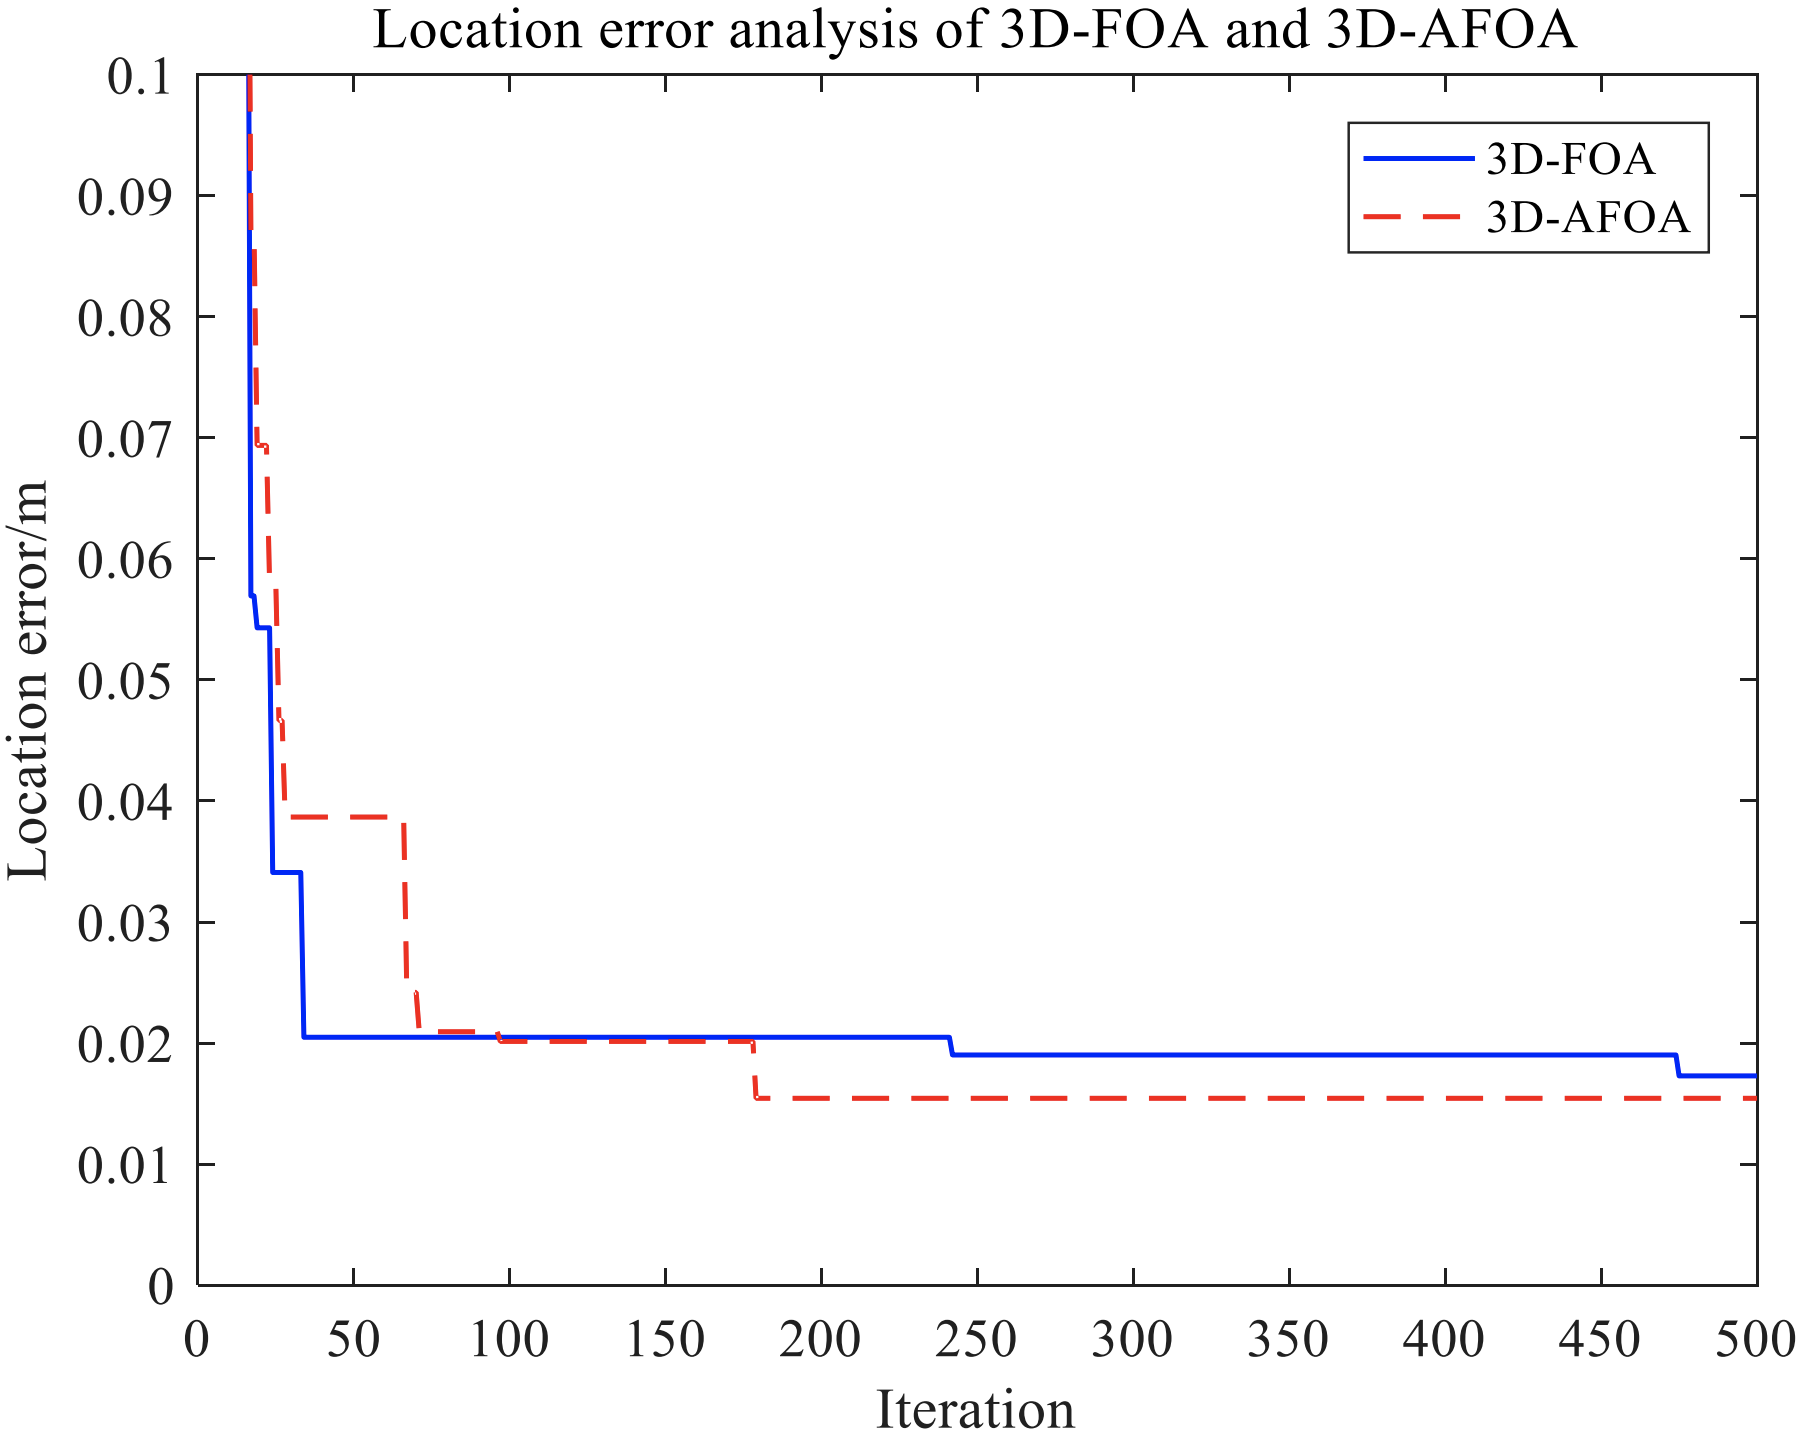
\includegraphics[width=\textwidth]{location-error-3d-foa-3d-afoa_1.png}
      \centering
      \caption{Resultados de error de detección de 3D-FOA y 3D-AFOA.}
      \label{fig:location-error-3d-foa-3d-afoa_1}
      \centering
    \end{figure}

    Como se puede ver en la figura \ref{fig:location-error-3d-foa-3d-afoa_1}, el
    algoritmo 3D-AFOA tiene un mejor desempeño, pues converge en una mejor
    solución en menos generaciones. 

    Cone l objetivo de verificar la efectividad del algoritmo, se probó con 3, 4
    y 5 nodos fijos en la red para detectar nuevamente un recurso en el taller
    simulado. Los resultados se muestran en \ref{fig:location-error-3d-afoa_2}.

    \begin{figure}[ht!]
      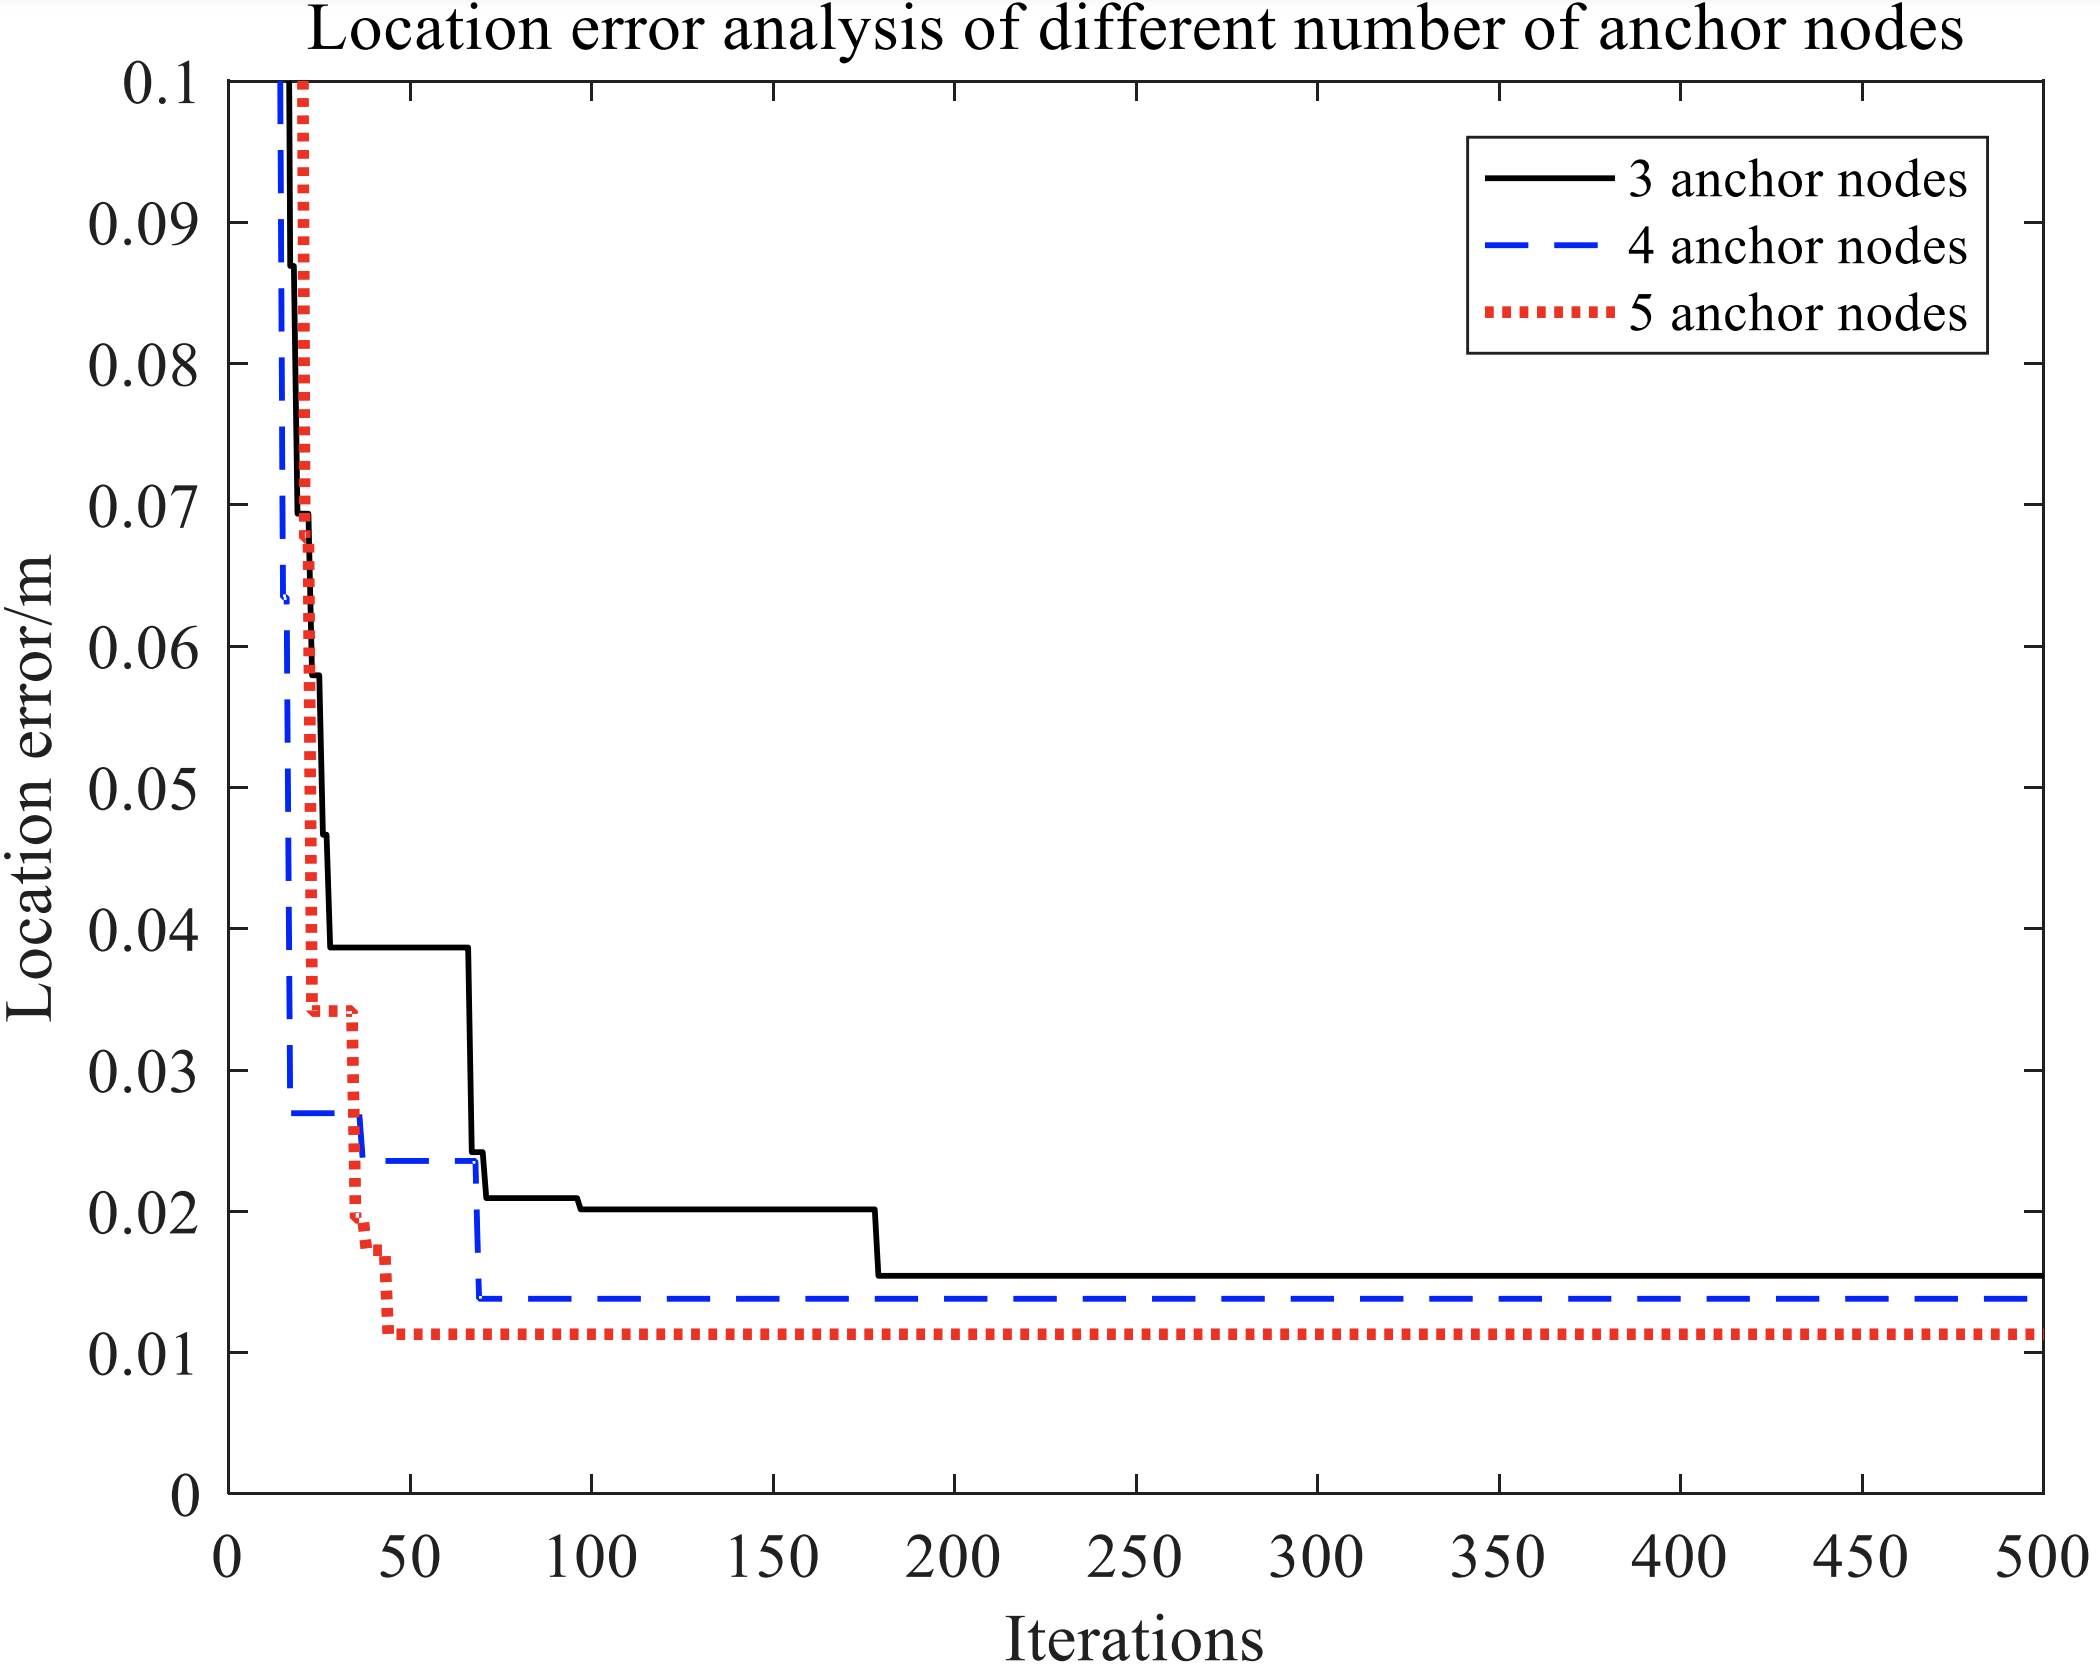
\includegraphics[width=\textwidth]{location-error-3d-afoa_2.png}
      \centering
      \caption{Resultados de error de detección con diferente cantidad de
        nodos.}
      \label{fig:location-error-3d-afoa_2}
      \centering
    \end{figure}

    Analizando los resultados expuestos en \ref{fig:location-error-3d-afoa_2},
    se puede apreciar que, conforme incrementa el número de nodos en el
    algoritmo, el tiempo de convergencia acelera. Sin embargo, el
    error de detección de los objetivos, aunque mejora con más nodos, no existe
    gran diferencia. Esto es debido a que solamente la ubicación de un solo nodo
    fue optimizada en los algoritmos. 

    Para finalizar, los investigadores concluyeron que 3D-AFOA es altamente
    aplicable al problema de optimización en la ubicación de nodos en una red
    WSN y no requiere de un alto presupuesto computacional para lograr buenas
    soluciones. 

  \subsection{Asignación óptima de unidades de generación distribuidas en
    sistemas de energía radiales}
    Como segundo trabajo relevante presentado en esta sección, Hantash et al,
    en 2020 \cite{PSOEnergy}, publicaron un estudio en el que
    proponen una modificación al estándar PSO-iw para calcular las posiciones y
    tamaños de unidades generadoras distribuidas en una red radial de energía
    eléctrica. 

    Los autores partieron del estándar PSO-iw y, después de una investigación,
    encontraron que valores grandes en el peso inercial ($w$) facilitan la
    búsqueda global, mientras que valores pequeños de $w$ favorecen la búsqueda
    local \cite{CPSO, APSO2016}. Gracias a estos hallazgos, los autores proponen
    una estrategia no
    lineal para obtener valores de $w$ variables con el tiempo. Esta estrategia
    está descrita en la Ecuación \ref{eq:4}:

    \begin{equation}
      \label{eq:4}
      w = w_{max} e^{(((maxiter - iter) / maxiter) - 1)} - w_{min} 
    \end{equation}
    en donde $w_{max}$ es el peso máximo, $w_{min}$ es el peso mínimo, $iter$ es
    la iteración actual y $maxiter$ es el número máximo de iteraciones.

    Finalmente, para validar sus resultados, el grupo de investigadores
    decidió comparar su
    estrategia propuesta contra un PSO convencional. Para comparar los
    resultados arrojados por ambos algoritmos, se usó la red de energía estándar
    IEEE 34. Después de la ejecución de los experimentos, los investigadores
    obtuvieron pérdidas de energía 31.6\% menores con su propuesta de PSO a
    comparación del PSO convencional sin el valor de $w$ variable. Además de
    esto, la propuesta consumió 62.2325 s para proveer una solución optima,
    cuando el PSO convencional consumió 62.2325 s. La comparación completa
    entre el PSO propuesto y el convencional está en la Figura
    \ref{fig:pso-iw-variable-comp}.

    \begin{figure}[ht!]
      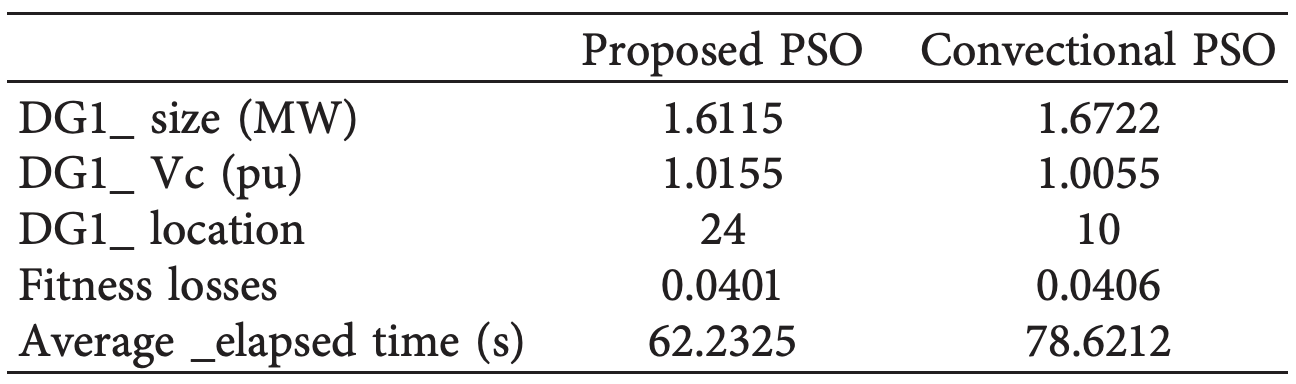
\includegraphics[width=\textwidth]{pso-iw-variable-comp.png}
      \centering
      \caption{Comparación de resultados entre el PSO propuesto y el
        convencional.}
      \label{fig:pso-iw-variable-comp}
      \centering
    \end{figure}

  \subsection{Optimización de ubicación de trampas para mosquitos}
    \label{subsection:mgsurve}
    Para finalizar esta sección, se describe el
    trabajo realizado por Sánchez y el Departamento de bioestadística y
    epidemiología de la universidad de Berkley \cite{MGSurvE} que aún no ha sido
    publicado y sigue en progreso, sin embargo, es el estado del arte en el área
    de este trabajo. Sánchez et al están trabajando en un paquete llamado
    MGSurvE, el cual está diseñado para optimizar la ubicación de trampas de
    mosquito en entornos espacialmente heterogéneos. 

    En el estado actual del paquete cuenta con diversas funcionalidades, tales
    como: diferentes kernels de movimiento para mosquitos machos y hembras;
    kernels de atractivo para trampas personalizables; soporte para trampas
    inamovibles; rutinas de trazado de mapas integradas; integración de rutinas
    para optimización con GA; y mucho más, con más funciones esperadas en
    futuras actualizaciones.

    Como se mencionó, las rutinas de optimización para la ubicación de las
    trampas para mosquito se implementa un algoritmo genético (GA), el cual es
    la variante estándar y es importado directamente del paquete DEAP
    \cite{DEAP}.

    Para el correcto funcionamiento del algoritmo de optimización, 3 grupos de
    características deben ser definidas: del entorno, de las trampas y del
    comportamiento de migración de mosquitos. En la figura
    \ref{fig:mgsurve-landscape-diagram} se describe cómo estos tres grupos de
    características forman el "Landscape", el cual es usado por el algoritmo 
    genético. 

    \begin{figure}[ht!]
      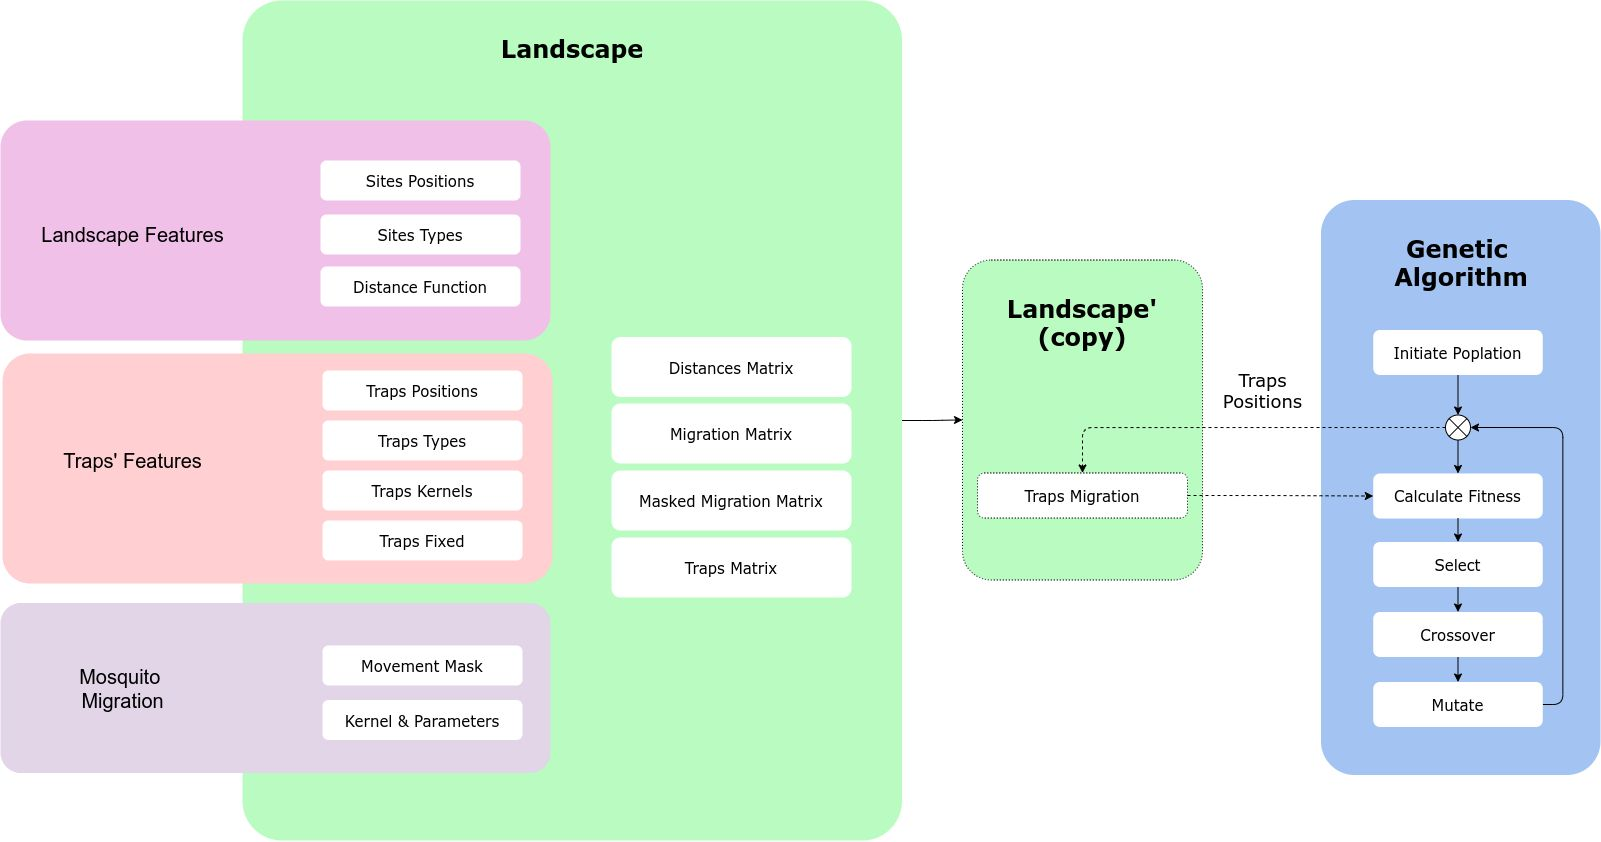
\includegraphics[width=\textwidth]{fig:mgsurve-landscape-diagram.jpeg}
      \centering
      \caption{Interacción del Landscape con el algoritmo genético.}
      \label{fig:mgsurve-landscape-diagram}
      \centering
    \end{figure}

    En la fecha de realización de este capítulo, aunque no hay ningún
    experimento publicado oficialmente, la documentación del paquete sí cuenta
    con ejemplos y tutoriales de optimización en la siguiente URL
    \url{https://chipdelmal.github.io/MGSurvE/build/html/GA.html}. En los
    tutoriales, el número de población es de 10 por cada trampa a optimizar. Si
    se desean optimizar 4 trampas, se utiliza una población de entre 40 o 50.
    Además de definir la población, también se limita a 500 generaciones para
    la optimización.

    Para finalizar, el paquete permite obtener el mejor cromosoma y trazar en un
    diagrama el mapa de las trampas y la migración de los mosquitos.

\section{Comparación de algoritmos}
  \label{section:analisis}
  Los trabajos mencionados en la sección anterior proponen diferentes algoritmos
  para solucionar problemas muy similares: encontrar la mejor ubicación de nodos
  en una red de nodos para optimizar algún resultado de una medición. Un aspecto
  en común de las soluciones propuestas por los diferentes investigadores es que
  todos hacen uso de algoritmos metaheurísticos iterativos para optimización.
  Otra similitud es que sus soluciones están basadas en inteligencia de enjambre
  y más específicamente en PSO. 

  Para resaltar las ventajas y desventajas de los diferentes tipos de
  algoritmos, en la tabla \ref{table:pso-ga-pros-cons} se muestra una
  comparación detallada entre PSO y GA.

  \begin{figure}[ht!]
    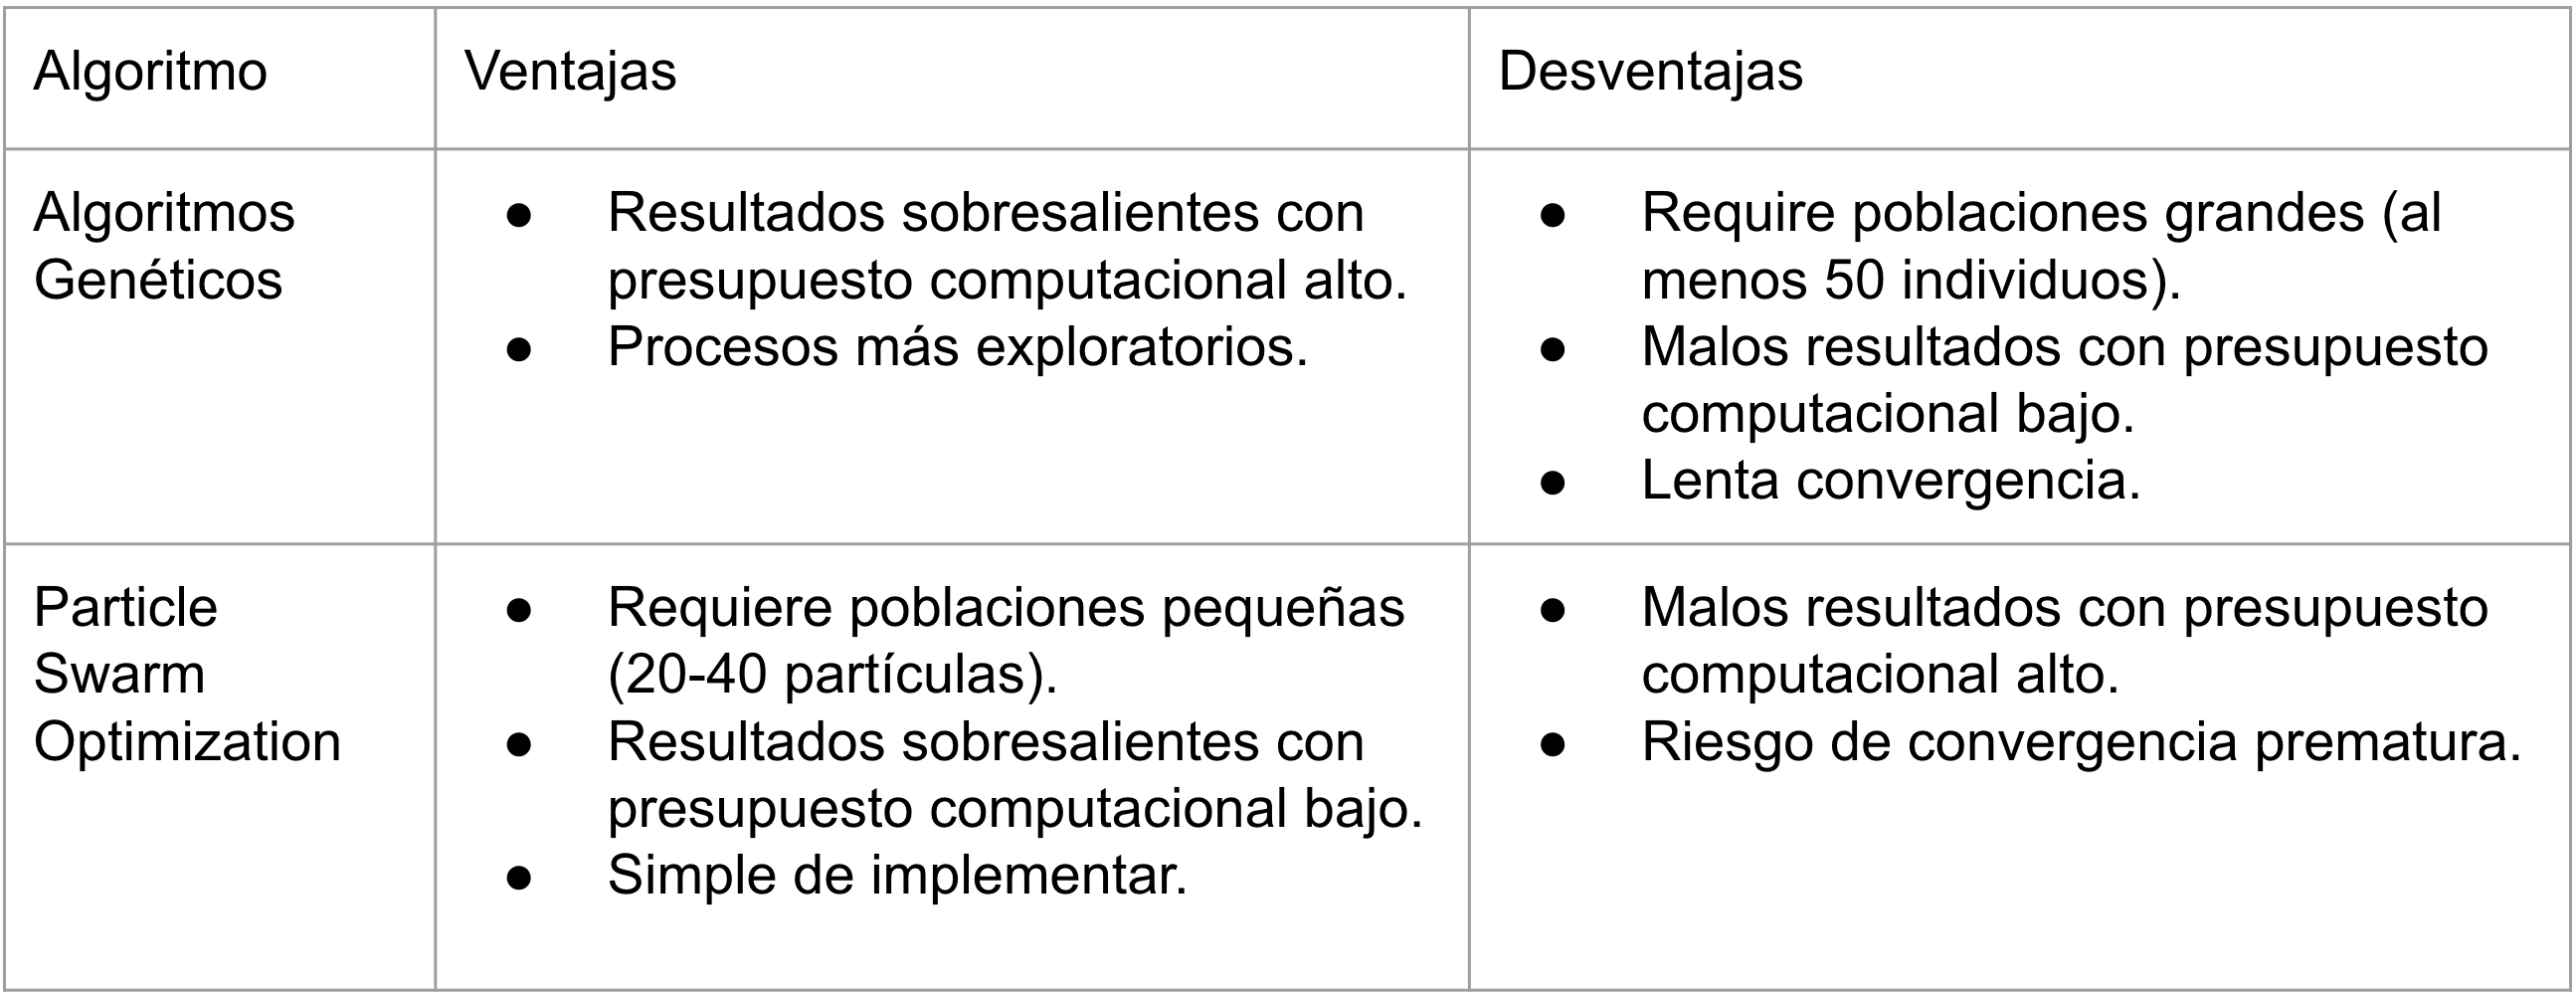
\includegraphics[width=\textwidth]{pso-ga-pros-cons.png}
    \caption{Ventajas y desventajas de PSO y GA basado en
      \cite{DE&PSOCov, SwarmVsEvol}.}
    \label{table:pso-ga-pros-cons}
  \end{figure}

  Además de los algoritmos propuestos por las investigaciones mencionadas en la 
  sección anterior, se pueden encontrar una gran variedad usados en la
  actualidad para 
  resolver problemas optimización. En un estudio realizado en 2021 por
  Piotrowski et al \cite{DE&PSOCov}, encontraron que las principales familias de
  algoritmos usados para resolver problemas de optimización relacionados a la 
  pandemia de COVID-19 fueron Swarm Intelligence (SI) y Evolutionary Algorithms
  (EA). 

  En 2017, un estudio similar realizado por Piotrowski et al \cite{SwarmVsEvol},
  sometieron a 33 metaheurísticas propuestas entre 1960 y 2016 a 22
  experimentos, cada una con diferentes presupuestos computacionales.
  Al finalizar los experimentos, encontraron que algoritmos basados en
  inteligencia de enjambre tienen un mejor desempeño cuando el presupuesto
  computacional es bajo. A diferencia de los algoritmos basados en inteligencia
  de enjambre, los basados en procesos evolutivos tienen un mejor desempeño
  cuando el presupuesto computacional es alto. 
  
  Aunque lo anterior es cierto, en un estudio de 2020 realizado por Piotrowski
  et al \cite{PSOPopulationSize}, se encontró que variantes modernas de PSO y
  SI sin peso inercial
  logran mejores resultados con una población de entre 70 y 500 partículas,
  contradiciendo las recomendaciones para lograr mejores resultados con
  variantes clásicas.
  Debido a esto, es de gran importancia conocer las condiciones adecuadas para
  cada variante de algoritmos basados en PSO. Si la cantidad adecuada de
  partículas para un problema en cuestión es desconocido, la recomendación es
  usar entre 70 y 100 partículas.

\section{Conclusión}
  En la actualidad, existe una gran variedad de algoritmos de optimización los
  cuales tienen comportamientos diferentes para cada tipo de problema
  \cite{SwarmVsEvol}. Por esto, es de suma importancia escoger correctamente el
  algoritmo que será empleado en alguna solución, para así obtener resultados
  realmente óptimos.

  Como se ve en la tabla \ref{table:pso-ga-pros-cons} y se discutió en la
  sección anterior, los algoritmos genéticos tienen un mejor comportamiento y
  desempeño cuando el presupuesto computacional y la población es grande
  (más de 50), por lo que el trabajo realizado en MGSurvE \cite{MGSurvE} no
  está optimizando correctamente las ubicaciones de las trampas para mosquitos,
  pues usan poblaciones de entre 40 y 50, además de un presupuesto computacional
  bajo. Esta situación da paso a una oportunidad de mejora, para implementar un
  algoritmo que se ajuste en mejor manera a la situación de MGSurvE, con la
  posibilidad de mejorar la optimización de la ubicación de las trampas para
  mosquitos.

\chapter{Planteamiento del problema}
  Después de analizar diferentes métodos de optimización aplicados en el área de
  este trabajo, el objetivo de este capítulo es describir la problemática en
  la optimización de la ubicación de trampas para mosquito. Para lograrlo, en
  este 
  capítulo primeramente se dará un poco de contexto sobre la herramienta actual,
  enseguida se hablará sobre problemas y limitaciones con la herramienta actual
  y finalmente se concluirá con el planteamiento del problema.

  \section{Contexto}
    \subsection{Marshall Lab}
    Marshall Lab \cite{MarshallLab} es un laboratorio perteneciente al
    departamento de epidemiología y bioestadística de la universidad de Berkeley
    en California. Su principal contribución es el desarrollo y simulación de
    estrategias basadas en genética para controlar enfermedades transmitidas por
    mosquitos. Para controlar estas enfermedades, el laboratorio simula la
    liberación de mosquitos modificados genéticamente en un entorno controlado,
    para así estudiar y desarrollar estrategias que permitan el comportamiento
    deseado de estos mosquitos en el ambiente. El control de los mosquitos
    liberados se hace con un correcto entendimiento de los patrones de
    movimiento de estos mosquitos. Para detectar el movimiento de mosquitos, se
    utilizan trampas, las cuales detectan la migración de los mosquitos.

    Para la simulación del correcto posicionamiento de trampas, el laboratorio
    ha creado el software MGSurvE \cite{MGSurvE}, el cual ya fue descrito en el
    capítulo anterior \ref{subsection:mgsurve}.

    Es de suma importancia el trabajo realizado por este laboratorio, pues el
    correcto posicionamiento de trampas para mosquitos significaría un ahorro
    económico en la batalla para el control de enfermedades transmitidas por
    mosquito.

  \section{Limitaciones de la herramienta actual}
    En la sección de comparación de algoritmos del capítulo del
    estado del arte
    \ref{section:analisis} se analizaron diferentes tipos de algoritmos de
    optimización y en la tabla \ref{table:pso-ga-pros-cons} se compararon los
    algoritmos de la familia de PSO contra algoritmos de la familia de GA. Se
    concluyó en esa sección que los algoritmos PSO generalmente tienen un mejor
    desempeño cuando el presupuesto computacional es bajo, lo contrario de
    algoritmos de tipo GA. Como se habló en la sección \ref{subsection:mgsurve},
    el paquete MGSurvE implementa un algoritmo genético (GA) para sus tareas de
    optimización de tiempos de detección de mosquitos. Sin embargo, se hace uso
    de una población pequeña, así como un límite de 500 generaciones, por lo que
    el presupuesto computacional es bajo y el rendimiento del algoritmo y sus
    resultados obtenidos posiblemente no sean los óptimos.

  \section{Conclusión}
    Después de establecer un estado del arte en el capítulo anterior y detallar
    las limitaciones de la herramienta actual, se puede concluir la problemática
    como: El software MGSurvE no genera las ubicaciones óptimas para trampas de
    mosquitos. 

\chapter{Solución}
  En este capítulo se detalla la solución propuesta para la problemática
  expuesta en el capítulo anterior. Se explica el diseño y desarrollo de la
  solución, así como el algoritmo implementado y configuración de
  hyperparámetros.

  \section{Diseño de la solución}
    \subsection{Selección de algoritmo}
    Como se habló en el capítulo pasado, la problemática a resolver es que el
    paquete MGSurvE no genera las ubicaciones óptimas para trampas de mosquitos.
    siendo la causa principal del
    problema que el algoritmo de optimización usado actualmente en MGSurvE
    (un algoritmo genético, o GA) no tiene un correcto comportamiento con el
    bajo presupuesto computacional \cite{SwarmVsEvol}. Por esto, un algoritmo
    perteneciente a
    la familia de Particle Swarm Optimization (PSO) es adecuado para resolver
    este problema \cite{SwarmVsEvol,PSOPopulationSize}. Los algoritmos de tipo
    PSO tienden a comportarse de manera ideal con una población pequeña (de 3
    a 40 partículas), por lo que necesitan un presupuesto computacional bajo,
    adecuado para resolver el problema presentado anteriormente.

    Se implementaron dos algoritmos como candidatos para la solución de la
    problemática. El primero, y más simple, es el PSO original propuesto
    por Kennedy y  Eberhart en \cite{PSODef}. Este algoritmo se divide en dos
    partes principales: la primera, actualización de la velocidad y posición de
    una partícula; y segunda, la evaluación de la función de aptitud y
    actualización de valores óptimos. Las partes del algoritmo están detalladas
    en las ecuaciones \ref{eq:pso-simple-update-1}, \ref{eq:pso-simple-update-2}
    y en el algoritmo \ref{alg:pso-simple-eval-1}.

    \begin{equation}
      v_{ij} = v_{ij} + c_1 rand()(p_{ij} - x_{ij}) + c_2 rand()(p_{nj}
        - x_{ij})
      \label{eq:pso-simple-update-1}
    \end{equation}

    \begin{equation}
      x_{ij} = x_{ij} + v_{ij}
      \label{eq:pso-simple-update-2}
    \end{equation}

    \begin{algorithm}
      \begin{algorithmic}
        \State Initialize $mejorParticula \gets None$
        \ForEach{$generacion \in generaciones$}
          \ForEach{$particula \in particulas$}
            \State $particula.aptitud.valores \gets funcionAptitud(particula)$

            \If {not $particula.mejor$ or $particula.mejor.aptitud < particula.aptitud$}
              \State $particula.mejor \gets$ nueva particula basada en $particula$
              \State $particula.mejor.aptitud.valores \gets particula.aptitud.valores$
            \EndIf

            \If {not $mejorParticula$ or $particula.aptitud < particula.aptitud$}
              \State $mejorParticula \gets$ nueva particula basada en $particula$
              \State $mejorParticula.aptitud.valores \gets particula.aptitud.valores$
            \EndIf
          \EndFor 

          \ForEach{$particula \in particulas$}
            \State $actualizaParticula(particula, mejorParticula)$
          \EndFor
        \EndFor
        \caption{Evaluación de función de aptitud y actualización de mejor
          partícula}
        \label{alg:pso-simple-eval-1}
      \end{algorithmic}
    \end{algorithm}

    Las ecuaciones \ref{eq:pso-simple-update-1} y \ref{eq:pso-simple-update-2}
    corresponden a la primer parte del PSO. En la primer ecuación, se realiza la
    actualización de la velocidad de la partícula $i$ en la o $j$ con
    respecto a la mejor partícula $n$. La segunda ecuación describe la
    actualización de la posición de la partícula con la nueva velocidad
    calculada. El algoritmo \ref{alg:pso-simple-eval-1} corresponde a la segunda
    parte del algoritmo.

    El segundo algoritmo candidato como solución del problema es el propuesto
    en 2020 por Hantash et al \cite{PSOEnergy}. En este algoritmo introducen una
    variación al peso inercial original propuesto por Shi et al \cite{CPSO} en
    1998 (descrito anteriormente en la sub sección \ref{subsec:pso}). Con esta
    modificación la convergencia del algoritmo es controlada por el peso. Al 
    empezar con valores mayores y terminar con valores menores, se prioriza la
    búsqueda global inicialmente y, en las últimas etapas de la búsqueda, se
    prioriza una búsqueda local en cada partícula \cite{CPSO}.

    \begin{equation}
      \label{eq:pso-weight-update}
      w = w_{max} e^{(((maxiter - iter) / maxiter) - 1)} - w_{min} 
    \end{equation}

    En la ecuación \ref{eq:pso-weight-update} se muestra el cálculo y
    actualización del peso inercial. Al ser una función no lineal, se aseguran
    valores de $w$ más grandes en etapas tempranas de la búsqueda, así como
    rápida transición a valores más pequeños conforme progresa la búsqueda. Por
    lo tanto, se asegura una búsqueda global de mínimos con pocas posibilidades
    de quedar en un mínimo local \cite{APSO2016}. Al aplicar esta variación, la
    ecuación de actualización de velocidad de una partícula queda descrita en
    la ecuación \ref{eq:pso-variant-update}. La actualización de posición no se
    ve modificada (ecuación \ref{eq:pso-simple-update-2}) y el algoritmo de
    que evalúa la función de aptitud sufre mínimas variaciones, descritas
    en el algoritmo \ref{alg:pso-variant-eval}.

    \begin{equation}
      v_{ij} = w v_{ij} + c_1 rand()(p_{ij} - x_{ij}) + c_2 rand()(p_{nj}
        - x_{ij})
      \label{eq:pso-variant-update}
    \end{equation}

    \begin{algorithm}
      \begin{algorithmic}
        \State Initialize $mejorParticula \gets None$
        \ForEach{$generacion \in generaciones$}
          \ForEach{$particula \in particulas$}
            \State $particula.aptitud.valores \gets funcionAptitud(particula)$

            \If {not $particula.mejor$ or $particula.mejor.aptitud < particula.aptitud$}
              \State $particula.mejor \gets$ nueva particula basada en $particula$
              \State $particula.mejor.aptitud.valores \gets particula.aptitud.valores$
            \EndIf

            \If {not $mejorParticula$ or $particula.aptitud < particula.aptitud$}
              \State $mejorParticula \gets$ nueva particula basada en $particula$
              \State $mejorParticula.aptitud.valores \gets particula.aptitud.valores$
            \EndIf
          \EndFor 

          \ForEach{$particula \in particulas$}
            \State $actualizaParticula(particula, mejorParticula, generacion)$
          \EndFor
        \EndFor
        \caption{Evaluación de función de aptitud y actualización de mejor
          partícula}
        \label{alg:pso-variant-eval}
      \end{algorithmic}
    \end{algorithm}

    \subsection{Stack tecnológico}
    MGSurvE, al ser un paquete para ser usado en proyectos desarrollados con el
    lenguaje de programación Python, da la oportunidad de usar una gran variedad
    de paquetes, bibliotecas y Frameworks indexadas en el PyPI. A continuación
    se describe la lista completa de dependencias usadas para la implementación
    de los algoritmos.

    Como herramienta principal para la manipulación de datos está la biblioteca
    Pandas \cite{PandasDocs}. Esta herramienta de código libre permite el
    análisis y manipulación de datos en la solución, así como la creación de
    gráficas rápida y sencillamente.

    Además de análisis y manipulación de datos, la solución depende de una
    herramienta que permite realizar operaciones con vectores y matrices. El
    paquete por default en el ecosistema de Python es NumPy, el cual ofrece
    funciones matemáticas y de vectorización. Escrito en código optimizado de C
    y con una interfaz para Python, ofrece gran eficiencia y oportunidades de 
    paralelización en sus operaciones \cite{NumPyDocs}.

    Por último, para la implementación del algoritmo se basa en el paquete DEAP
    \cite{DEAPDocs}, el cual provee un marco de trabajo para la creación e
    implementación de algoritmos evolutivos en Python. La implementación del
    algoritmo genético con el que funciona actualmente MGSurvE está construida
    con DEAP, por lo que la reutilización de este paquete ayuda el desarrollo de
    la solución propuesta en este trabajo.

% \chapter{Metodología de evaluación}

% \chapter{Resultados y contribuciones}

% \chapter{Conclusiones}

\begin{thebibliography}{99}
  \bibitem{AIModernAproach}S. Russell and P. Norving, “Artificial Intelligence: A modern approach”, 3rd ed. Prentice Hall, New Jersey: Pearson Education, 2009. 
  \bibitem{AIDef}J. M. Spector and S. Ma, “Inquiry and critical thinking skills for the next generation: From Artificial Intelligence back to human intelligence,” Smart Learning Environments, vol. 6, no. 1, Sep. 2019. 
  \bibitem{SearchMethodologies}E. K. Burke and G. Kendall, “Search methodologies: Introductory tutorials in optimization and decision support techniques”. New York, New York: Springer, 2014.
  \bibitem{HeuristicDef}V. J. Rayward-Smith, “Modern Heuristic Search Methods”. Chichester, New York: Wiley, 1996. 
  \bibitem{MetaheuristicsDef}F. Glover and M. Laguna, “Tabu Search”. Boston, Massachusets: Kluwer Academic Publishers, 1997.
  \bibitem{EADef}C. A. Coello Coello, G. B. Lamont, and D. A. Van Veldhuizen, “Evolutionary algorithms for solving multi-objective problems,” Genetic and Evolutionary Computation Series, 2007. 
  \bibitem{GADef}A. S. Fraser, “Simulation of genetic systems by Automatic Digital Computers II. effects of linkage on rates of advance under selection,” Australian Journal of Biological Sciences, vol. 10, no. 4, p. 492, 1957. 
  \bibitem{PSODef}J. Kennedy and R. Eberhart, “Particle swarm optimization,” Proceedings of ICNN'95 - International Conference on Neural Networks, 1995. 
  \bibitem{CPSO}Y. Shi and R. Eberhart, “A modified particle swarm optimizer,” 1998 IEEE International Conference on Evolutionary Computation Proceedings. IEEE World Congress on Computational Intelligence (Cat. No.98TH8360), 1998. 
  \bibitem{PSOReview}S. Cheg, H. Lu, X. Lei, and Y. Shi, “A quarter century of particle swarm optimization,”, Complex and Intelligent Systems, vol. 4, no. 3, pp. 227 239, 2018.

  \bibitem{3DAFAO}S. Li, C. Zhang, and J. Qu, “Location optimization of wireless sensor network in Intelligent Workshop based on the three-dimensional adaptive fruit fly optimization algorithm,” International Journal of Online Engineering (iJOE), vol. 14, no. 11, p. 202, Nov. 2018. 
  \bibitem{PSOEnergy}N. Hantash, T. Khatib, and M. Khammash, “An improved particle swarm optimization algorithm for optimal allocation of distributed generation units in Radial Power Systems,” Applied Computational Intelligence and Soft Computing, vol. 2020, pp. 1-8.
  \bibitem{APSO2016}H. Liang and F. H. Kang, “Adaptive mutation particle swarm algorithm with dynamic nonlinear changed inertia weight,” Optik-International Journal for Light and Electron Optics, vol. 127, no. 19, pp. 8036-8042, 2016.
  \bibitem{MGSurvE}H. M. Sanchez, “MGSurvE's documentation,” MGSurvE's documentation! - MGSurvE documentation, 2021. [Online]. Available: https://chipdelmal.github.io/MGSurvE/build/html/index.html. [Accessed: 31-Mar-2022]. 
  \bibitem{DEAP}DEAP Project, “DEAP documentation,” DEAP documentation - DEAP 1.3.1 documentation, 2022. [Online]. Available: https://deap.readthedocs.io/en/master/. [Accessed: 01-Apr-2022]. 
  \bibitem{DE&PSOCov}A. P. Piotrowski and A. E. Piotrowska, “Differential Evolution and particle swarm optimization against covid-19,” Artificial Intelligence Review, Jul. 2021. 
  \bibitem{SwarmVsEvol}A. P. Piotrowski, M. J. Napiorkowski, J. J. Napiorkowski, and P. M. Rowinski, “Swarm intelligence and Evolutionary Algorithms: Performance versus speed,” Information Sciences, vol. 384, pp. 34-85, Apr. 2017. 
  \bibitem{PSOPopulationSize}A. P. Piotrowski, J. J. Napiorkowski, and A. E. Piotrowska, “Population size in particle swarm optimization,” Swarm and Evolutionary Computation, vol. 58, May 2020. 
  \bibitem{MarshallLab}The Marshall Lab at UC Berkeley. (s. f.). THE MARSHALL LAB. https://www.marshalllab.com/

  \bibitem{ShapeUp}R. Singer, “Shape up V 1.8, 2019 edition,” Shape Up: Stop Running in Circles and Ship Work that Matters, 2019. [Online]. Available: https://basecamp.com/shapeup/webbook. [Accessed: 03-May-2022]. 
  \bibitem{PandasDocs}“Pandas,” pandas, 02-Apr-2022. [Online]. Available: https://pandas.pydata.org/. [Accessed: 06-May-2022]. 
  \bibitem{NumPyDocs}NumPy, 2022. [Online]. Available: https://numpy.org/. [Accessed: 06-May-2022]. 
  \bibitem{DEAPDocs}“DEAP documentation,” DEAP documentation - DEAP 1.3.1 documentation, 22-Jan-2022. [Online]. Available: https://deap.readthedocs.io/en/master/. [Accessed: 06-May-2022]. 
\end{thebibliography}

\end{document}
